\section{Implementation and Evaluation}
\label{sect-implem}



\subsection{\biptool{}} \label{chap:implementation:bip}
We implemented \biptool{} in JAVA and used the BIP parser provided 
freely in~\cite{verimagbiponline}. Given an input BIP program \Pm, 
the parser generates a parse graph $G$. \biptool{} traverses $G$ 
and translates \Pm into an equivalent \caig{} program 
\Pm'. We then use the same synthesis engine in \mytool{} to synthesize
an equisatisfiable AIG circuit \aigcircuit{} that is passed to ABC 
for sequential synthesis and verification.

\biptool{} is equipped with a command line interface that accepts a set
of configuration options. It takes the name of the input BIP file, optional 
configuration flags and an option to generate C++ emulation code. After 
parsing the input file, we perform synthesis steps and generates 
an output \caig{} file. 
We then pass this file to synthesize the AIG circuit \aigcircuit{}
and call ABC for reduction and verification. \biptool{} makes use of the same debugging
interface provided by \mytool{} in order to allow users to visualize counterexamples
if any is return by ABC. 

Additionally, \biptool{} supports the generation of C++ emulation code. It allows
the users to guide the execution engine by providing a guide file
that lists the order in which interactions are to take place. In case no such file 
is provided, the emulator uses a random number generator to choose an interaction to execute
in case several candidates  are available. \biptool{} also allows
users to set a bound on the number of clock cycles to execute in the emulation code. 
Furthermore, \biptool{} allows users to specify whether to initialize the variables 
in the atomic components or to leave them as free inputs. Figure~\ref{fig:implementation:bip}
shows \biptool's command line options along with their description and an example usage. 


\begin{lstlisting}[language=Bash]
# Usage #
> java -jar bip-to-abc.jar [options] input.bip output.abc [property.txt]

where:

  input.bip    = input BIP file name (required)
  output.abc   = ABC file name to be generated (required)
  property.txt = Pre and Post condition written in two different lines (optional)

and options are:

  -?                prints usage to stdout; exits (optional)  
  -emulator <s>     Generate emulation code output.abc.cpp (optional)  
                     - guide.txt: indices of interactions assigned to selector 
                     - integer <= 0: infinite exection 
                     - integer > 0: number of cycles to be executed 
  -h                prints usage to stdout; exits (optional) 
  -help             displays verbose help information (optional)
  -optimized        Generate one cycle-based code (optional)
  -initialize-vars  Initialize free variables (optional)
  -version          displays command's version (optional)
  
# Example #

> java -jar bip-to-abc.jar -optimized -initialize-vars -emulator=guide input.bip output.abc property.txt
> java -jar bip-to-abc.jar -o -i -e=guide input.bip output.abc property.txt
> java -jar bip-to-abc.jar -o -i -e=0 input.bip output.abc property.txt
> java -jar bip-to-abc.jar -o -i -e=30 input.bip output.abc property.txt  
> java -jar bip-to-abc.jar -o -e=guide input.bip output.abc
\end{lstlisting}



%% bip results
We evaluated \biptool{} against two industrial benchmarks, 
an {\em Automatic Teller Machine} (ATM)~\cite{atm} and the {\em Quorum} consensus
protocol~\cite{guerraoui2012speculative}. We report on the size of the generated
AIGs before and after reduction, and on the time taken by the ABC solver to 
reduce and verify the benchmarks. We compare the results for the 
verification of the ATM benchmark
with the NuSMV~\cite{nusmv} model checker.


\subsection{The ATM benchmark}
An ATM is a computerized system that provides financial services for users in 
a public space. 
%\textit{Automatic Teller Machine} (ATM) is a computerized telecommunication device
%that provides services to access to financial transactions in a public space without
%the need for a cashier, human clerk or bank teller.
Figure~\ref{fig:atm_bip} shows a structured BIP model of an ATM system adapted from the
description provided in~\cite{atm}.
The system is composed of four atomic components: (1) the User, (2) the ATM, (3) the Bank Validation 
and (4) the Bank Transaction. It is the job of the ATM component to handle all interactions between the 
users and the bank. No communication between the users and the bank is allowed. 
%The structural BIP model of an ATM system \cite{atm} is presented in Figure \ref{fig:atm_bip}.
%The system is composed of the following components: User, ATM (modeling a cash dispenser)
%and Bank (modeling some aspects of bank operation). User and Bank interact only with ATM,
%but not with each other.
\begin{figure}[bt]
 \centering
  %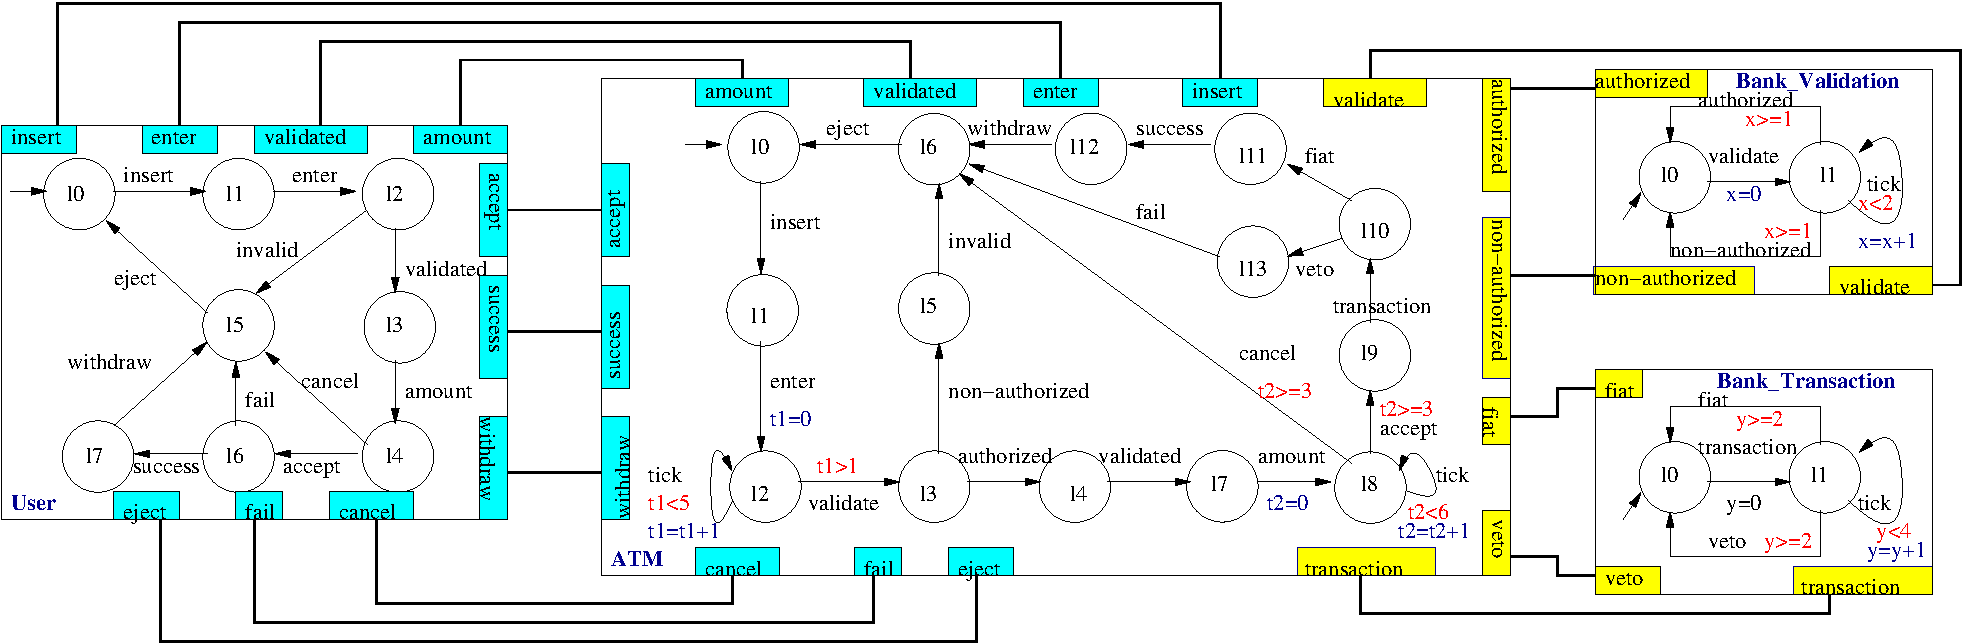
\includegraphics[width=1.0\textwidth]{figures/atm_bip.pdf}
  \resizebox{1.0\textwidth}{!}{
       \input{figures/atm_bip.pdftex_t}
  }
  \caption{Modeling of ATM system in BIP} \vspace*{-0.5cm}
  \label{fig:atm_bip}
% \end{center}
\end{figure}

The ATM starts from an idle location and waits for the user to insert his card 
and enter the confidential code. The user has $5$ time units
to enter the code before the counter expires and the card is ejected by the ATM. 
Once the code is entered, the ATM checks with the bank validation unit for 
the correctness of the code. If the code is invalid, the card is ejected
and no transaction occurs. If the code is valid, the ATM waits for the user to enter
the desired amount of money for the transaction. The time-out for entering the amount 
of money is of $6$ time units. 

Once the user enters the desired transaction amount, the ATM checks with the bank whether 
the transaction is allowed or not by communicating with the bank transaction unit.
If the transaction is approved, the money is transferred to the user and the card is ejected. 
If the transaction is rejected, the user is notified and the card is ejected. In all cases, 
the ATM goes back to the idle location waiting for any additional users. 
In our model, we assume the presence of a single bank and multiple ATMs and users. 

\begin{table}[tb]
\caption{ATM results}
\centering
\begin{tabular}{|c|c|c|c||c|c|c||c|c|}
\cline {2-9}
\multicolumn{1}{c|}{} &  \multicolumn{3}{c||}{Original} & \multicolumn{3}{c||}{After reduction} &  \multicolumn{2}{c|}{Time(s)} \\ \hline
ATMs & latches & and-gates & levels & latches & and-gates & levels & Verification Time & NuSMV \\ \hline
2 & 78 & 2308 & 125 & 37 & 552 & 25 & 26.1 & 1.4\\ \hline
3 & 102 & 3689 & 197 & 50 & 804 & 29 & 32.65 & 142.6 \\ \hline
4 & 146 & 5669 & 234 & 63 & 1036 & 29 &  597 & 3361 \\ \hline
\end{tabular}
\label{tb:bip:atm}
\end{table}

Table~\ref{tb:bip:atm} shows the improvement obtained by using \biptool{}
to verify the deadlock freedom of the ATM system, as compared to using the
NuSMV model checker~\cite{nusmv}.
The first column of the table shows the number of clients and ATMs in the system.
Columns \cci{lat}, \cci{and} and \cci{lev} present the number 
of latches, AND gates and logic levels in the AIG generated by \biptool{} before
and after applying reduction techniques, respectively.
We report on the verification time taken by the ABC solver to check the 
generated AIG, and the total taken to perform both synthesis (reduction) 
and verification, in addition to the time taken by NuSMV to perform verification.

With the increase in the number of users and ATMs in the system, \biptool{}  
outperforms NuSMV in terms of total verification time, reaching a speedup 
of $5.6$ for 4 users and ATMs. Additionally, \biptool{} allows developers
to make use of several reduction techniques that are able to reach an 
average of $50\%$ reduction in the size of the AIG. Note that for $2$ ATMs 
and users, NuSMV outperforms \biptool{}. This is due to the fact that when 
performing verification, ABC tries multiple verification and reduction 
algorithms before reaching a conclusive result. However, the advantage 
that \biptool{} presents can be clearly seen for larger number of ATMs and 
users. 


\subsection{The Quorum protocol}
The {\em Quorum} protocol is a consensus protocol proposed in~\cite{guerraoui2012speculative}
as complementary to the Paxos consensus protocol~\cite{gafni2003disk} under perfect
channel conditions. {\em Consensus} allows a set of communicating processes
(clients and servers in our case) to agree on a common value. Each of clients proposes
a value and receives a common decision value. The authors in~\cite{guerraoui2012speculative}
propose to use Quorum when no failures occur (perfect channel conditions) and 
Paxos when less than half of the servers may fail. 

The Quorum protocol operates as follows.
\begin{enumerate}
 \item Upon proposal, a client $c$ broadcasts its proposed value 
 $v$ to all servers. It also saves $v$ in its local memory and starts a local time
 $t_c$. 
 \item When a server receives a value $v$ from a client $c$, it performs
 the following check.
 \begin{itemize}
  \item It if has not sent any accept messages, it sends an accept message
  $accept(v)$ to the client $c$. 
  \item If it has already accepted value $v'$, it sends an accept message
  $accept(v')$ to the client $c$. 
 \end{itemize}
 \item If a client $c$ receives two different accept messages, it switches
 to the backup phase $switch-backup(proposal_c)$.
 \item If a client $c$ receives the same accept messages $accept(v)$ from all the servers,
 it decides on the value $v$.
 \item If a client's timer $t_c$ expires, it waits for at least
 one accept message $accept(v')$ from a server, or chooses a value $v'$
 from an already received $accept(v')$ message, and then switches to 
 the backup phase with the value $v'$. 
 \item The {\em backup} phase is an implementation of the Paxos algorithm. Quorum in this
 case has decided that the channel is not perfect. 
\end{enumerate}

We implemented the Quorum protocol in BIP, and we used \biptool{} to verify 
two invariants as defined in~\cite{guerraoui2012speculative}.
\begin{enumerate}
 \item[$Invariant_1$] If a client $c$ decides on a value $v$, then all clients 
 $c' \neq c$ that have switched, either before or after $c$, switch with the value $v$.
 \item[$Invarian_2$] If a client $c$ decides on a value $v$, then all clients
 $c' \neq c$ who decide, do so with the same value $v$. 
\end{enumerate}

Table~\ref{tb:bip:qrm} shows the results of using \biptool{} to verify the 
Quorum protocol for $2$ and $4$ clients with $2$ servers. The designs
are indexed as \cci{num\_clients}-\cci{num\_servers}-\cci{status} where 
\cci{num\_clients} is the number of clients, \cci{num\_servers} is the number of 
servers and \cci{status} is either valid (\cci{v}) or erroneous (\cci{e}).
A valid design contains no design bugs, while an errneous design is injected
with a bug. We report on the size of the AIG in terms of number of latches (\cci{lat}),
number of AND gates (\cci{and}) and logic levels (\cci{lev}) before and after
applying reduction algorithms. We also show the time taken by ABC to decide the problem, 
and the total time taken for reduction and decision procedures. 
A $\checkmark$ decision indicates that ABC proved that the property is never 
violated, \ie{} the design is valid, while a $\chi$ decision means that 
ABC was able to find a counter example that violates the property. 

\begin{table}[bt]
\caption{Quorum results}
\centering
\begin{tabular}{|c|c|c|c||c|c|c||c|c|}
\cline{2-9}
\multicolumn{1}{c|}{} & \multicolumn{ 3}{c||}{Original} & \multicolumn{3}{c||}{After reduction} & \multicolumn{ 2}{c|}{Time (s)} \\ \hline
Design & latches & and-gates & levels & latches & and-gates & levels & Verification Time & NuSMV \\ \hline
2-2-e & 264 & 3508 & 101 & 65 & 923 & 51 & 0.78 & 526 \\ \hline
2-2-v & 264 & 3614 & 105 & 66 & 641 & 29 & 240.6 & 526 \\ \hline
4-2-e & 390 & 6305 & 145 & 117 & 1129 & 50 & 0.24  & memory-out \\ \hline
4-2-v & 390 & 6453 & 151 & 117 & 1170 & 30 & 58 hours & memory-out \\ \hline
\end{tabular}
\label{tb:bip:qrm}
\end{table}

Using ABC's synthesis and reduction algorithms, \biptool{} was able to
reduce the size of the generated AIGs for all designs by a factor larger
than $50\%$. Furthermore,
\biptool{} was able to give conclusive results about all four designs, unlike
NuSMV which failed to give any decision about the designs having
$4$ clients and $2$ servers. For example, \biptool{} found a counter example for the erroneous 
design having $4$ clients and $2$ servers in $0.24 (s)$ while NuSMV failed to do
so. Figure~\ref{fig:res:counter} shows a snippet of the generated counter example for the 
erroneous design, visualized using the Gtkwave~\cite{bybell2010gtkwave} waveform viewer. 
The variables presented in the counterexample are the current control locations of
the different components in the design. 

\begin{figure}[bt]
\centering
\scalebox{0.75}{
 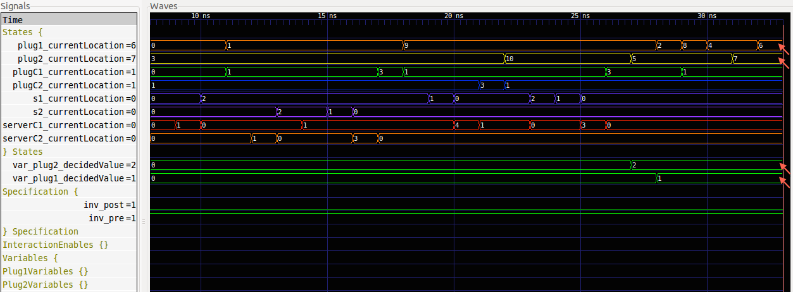
\includegraphics{figures/quorumDebug2}}
\caption{Visualization of a counter example using Gtkwave}
\label{fig:res:counter}
\end{figure}




